\section{Grundlagen}
\label{sec:basics}

\subsection{Markov Entscheidungsprozesse}
\label{sec:reinforcement}
\begin{figure}[h]
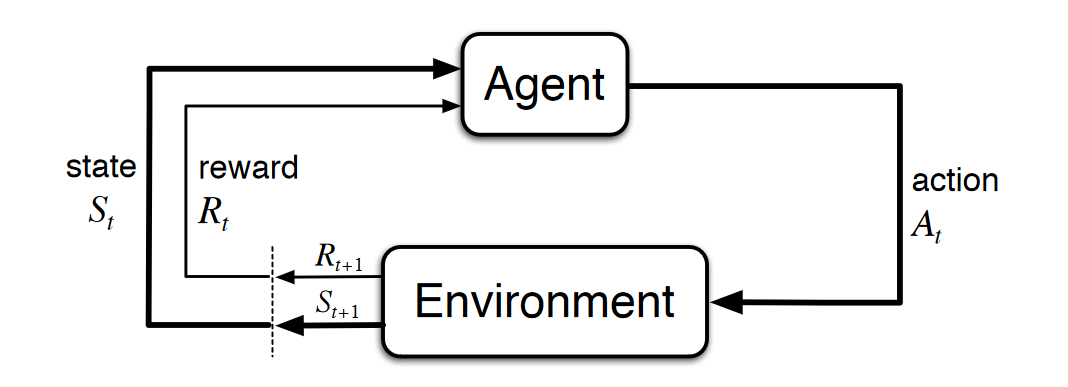
\includegraphics[width=\textwidth, keepaspectratio=true]{images/mdp.png}
\caption{Typischer Reinforcement Learning Zyklus} \label{img:rl_cycle}
\source{\cite{deeplizard_markov_decision_processes}}
\end{figure}
Das wohl elementarste Modell im Reinforcement Learning (RL) sind \textit{Markov Entscheidungsprozesse} (MDPs von engl. \textit{Markov Decision Processes}), hier erklärt nach \cite{deeplizard_markov_decision_processes}.

Ein MDP besitzt einen Entscheidungsträger, den so genannten \textit{Agenten} (im Folgenden auch als \textit{Aktor} bezeichnet), welcher mit seiner Umgebung (dem \textit{Environment}) interagiert. Diese Interaktion findet sequentiell statt. In jedem Zeitschritt $ t $ verfügt der Agent über eine Repräsentation seiner Umgebung, den Zustand oder auch \textit{State} $ S_t $. Aufgrund der dem Agenten vorliegenden Information wählt dieser eine Aktion $ A_t $. Dies führt dazu, dass das Environment in einen neuen Zustand $ S_{t+1} $ überführt wird. Außerdem erhält der Aktor von der Umgebung eine Belohnung $ R_{t+1} $, den \textit{Reward}.

Wie in \ref{img:rl_cycle} dargestellt findet dieser Prozess in einem andauernden Zyklus statt. Ziel des Agenten ist es, die Summe aller Rewards, die er für die Ausführung von Aktionen bekommt, zu maximieren. Sprich der Agent will nicht nur den folgenden Reward, sondern viel eher die Gesamtheit aller Rewards, die er auf Dauer bekommt, maximieren.

\subsection{TODO evtl Formeln zum MDP?}
\label{sec:markov}
